\subsubsection{Simulated Kitting into a Prismatic Target}
\label{subsubsec:prismatic}
\begin{figure}[t]
  \vspace{8pt}
  \centering
  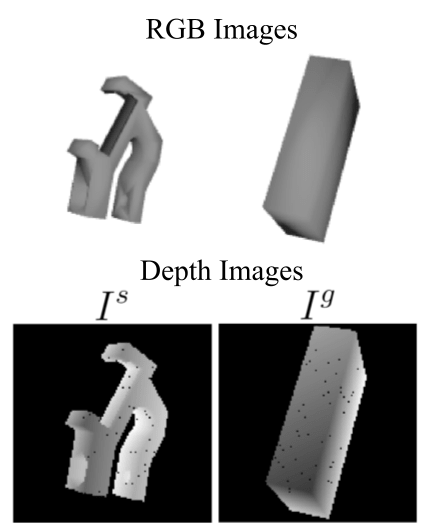
\includegraphics[width=0.8\linewidth]{figures/prismatic_example_labeled.png}
  \caption{\textbf{Endstop Holder and Target Prismatic Cavity in Simulation: } Given $I^s$, an image of an object in some configuration (top left) and $I^g$, an image of a target prismatic box to which the object must be aligned (top right), the objective is to find a 3D rotation $\hat{{_s}R^g}$ that would allow the object to fit within the box. In simulation experiments, $R^g$ is a $X$\degree~rotation from $R^s$, where $X\in (0,30)$. The image in the figure shows a 30\degree rotation, meaning the object must be rotated by 30\degree to perfectly fit it inside the prism. 3D models corresponding to $I^s$ and $I^g$ are shown in the bottom row for clarity. 
  }
  \label{fig:prism-task}
\end{figure}

We first study whether Kit-Net can orient objects into alignment with a prismatic cavity that loosely conforms to their 3D geometry in simulation. Precisely, we first generate the prismatic cavity for the target by creating a mesh with faces corresponding to its minimum volume bounding box. We then rotate both the prismatic cavity and target to random orientations within 30 degrees of each other. The objective is to apply a rotation ${_s}\hat{R}^g$ that will allow the object to fit into the cavity. An example image pair of an object and an associated prismatic cavity is shown in Figure~\ref{fig:prism-task}.

Fig.~\ref{fig:mean-percent-fit-ecc} shows the percent fit across 174 unseen test objects. We use the eccentricity $\epsilon$ of the objects to sort them into 5 bins of increasing difficulty (increasing $\epsilon$). We find that Kit-Net is able to reliably kit novel objects, significantly outperforming the 2D rotation baseline. When averaged across all eccentricities, Kit-Net achieves an average fit of 98.9\,\% compared to an average fit of 93.6\,\% for the 2D baseline and 83.1\,\% when applying a random 30\degree~quaternion. These results demonstrate the need for 3D rotations to solve complex kitting problems. Figure~\ref{fig:mean-percent-fit-ecc} demonstrates that Kit-Net is robust to highly eccentric objects which require the most precision for kitting. Kit-Net achieves an average fit of 89.9\,\% for objects with eccentricity greater than 8. The 2D rotation baseline performs especially poorly for these difficult objects and achieves an average fit of only 72.7\,\% while applying a random 30\degree~quaternion results in an average fit of just 37.4\,\%.

As described in Section~\ref{subsec:kit-net-alg}, Kit-Net iteratively orients each object using the controller until $\hat{{_s}R^g}\leq 5\degree~$ or until we hit the stopping condition of 8 rotations. Our previous results in Fig.~\ref{fig:mean-percent-fit-ecc} suggests that Kit-Net can consistently align objects within 5 controller steps.
To better visualize the ability of Kit-Net to rapidly reorient an object for kitting, we plotted the per-iteration performance of Kit-Net for 4 test objects unseen during training time with high eccentricity ($\epsilon \geq 2$).  Fig.~\ref{fig:prism-task-eval-objects} shows renderings of these objects along with outlines of the corresponding prismatic kitting cavities. Fig.~\ref{fig:percent-fit-runs} shows the average per-iteration percent fit across 100 controller rollouts of randomly sampled $(I^s,I^g)$ pairs for each object. We find that Kit-Net is able to consistently align objects with their target prismatic cavities, and achieves a median fit percentage of 99.4\,\% after only 3 successive reorientations. By contrast, the 2D baseline is not able to surpass an average fit of 90\,\% for any of the objects. The results in Fig.~\ref{fig:percent-fit-runs} validate the importance of iteratively reorienting parts and demonstrates that applying multiple iterations of the rotation output by the trained network can greatly help to reduce the error between $\hat{{_s}R^g}R^s$ and $R^g$ as compared to a single iteration. 
%DB{it would be nice to include a failure case here as well} 
% and for many objects, including the four shown in Figure~\ref{fig:prism-task-eval-objects}, Kit-Net achieves successful alignment in just 3 steps (Figure~\ref{fig:percent-fit-runs}).

\begin{figure}[t]
  \centering
  \vspace{8pt}
  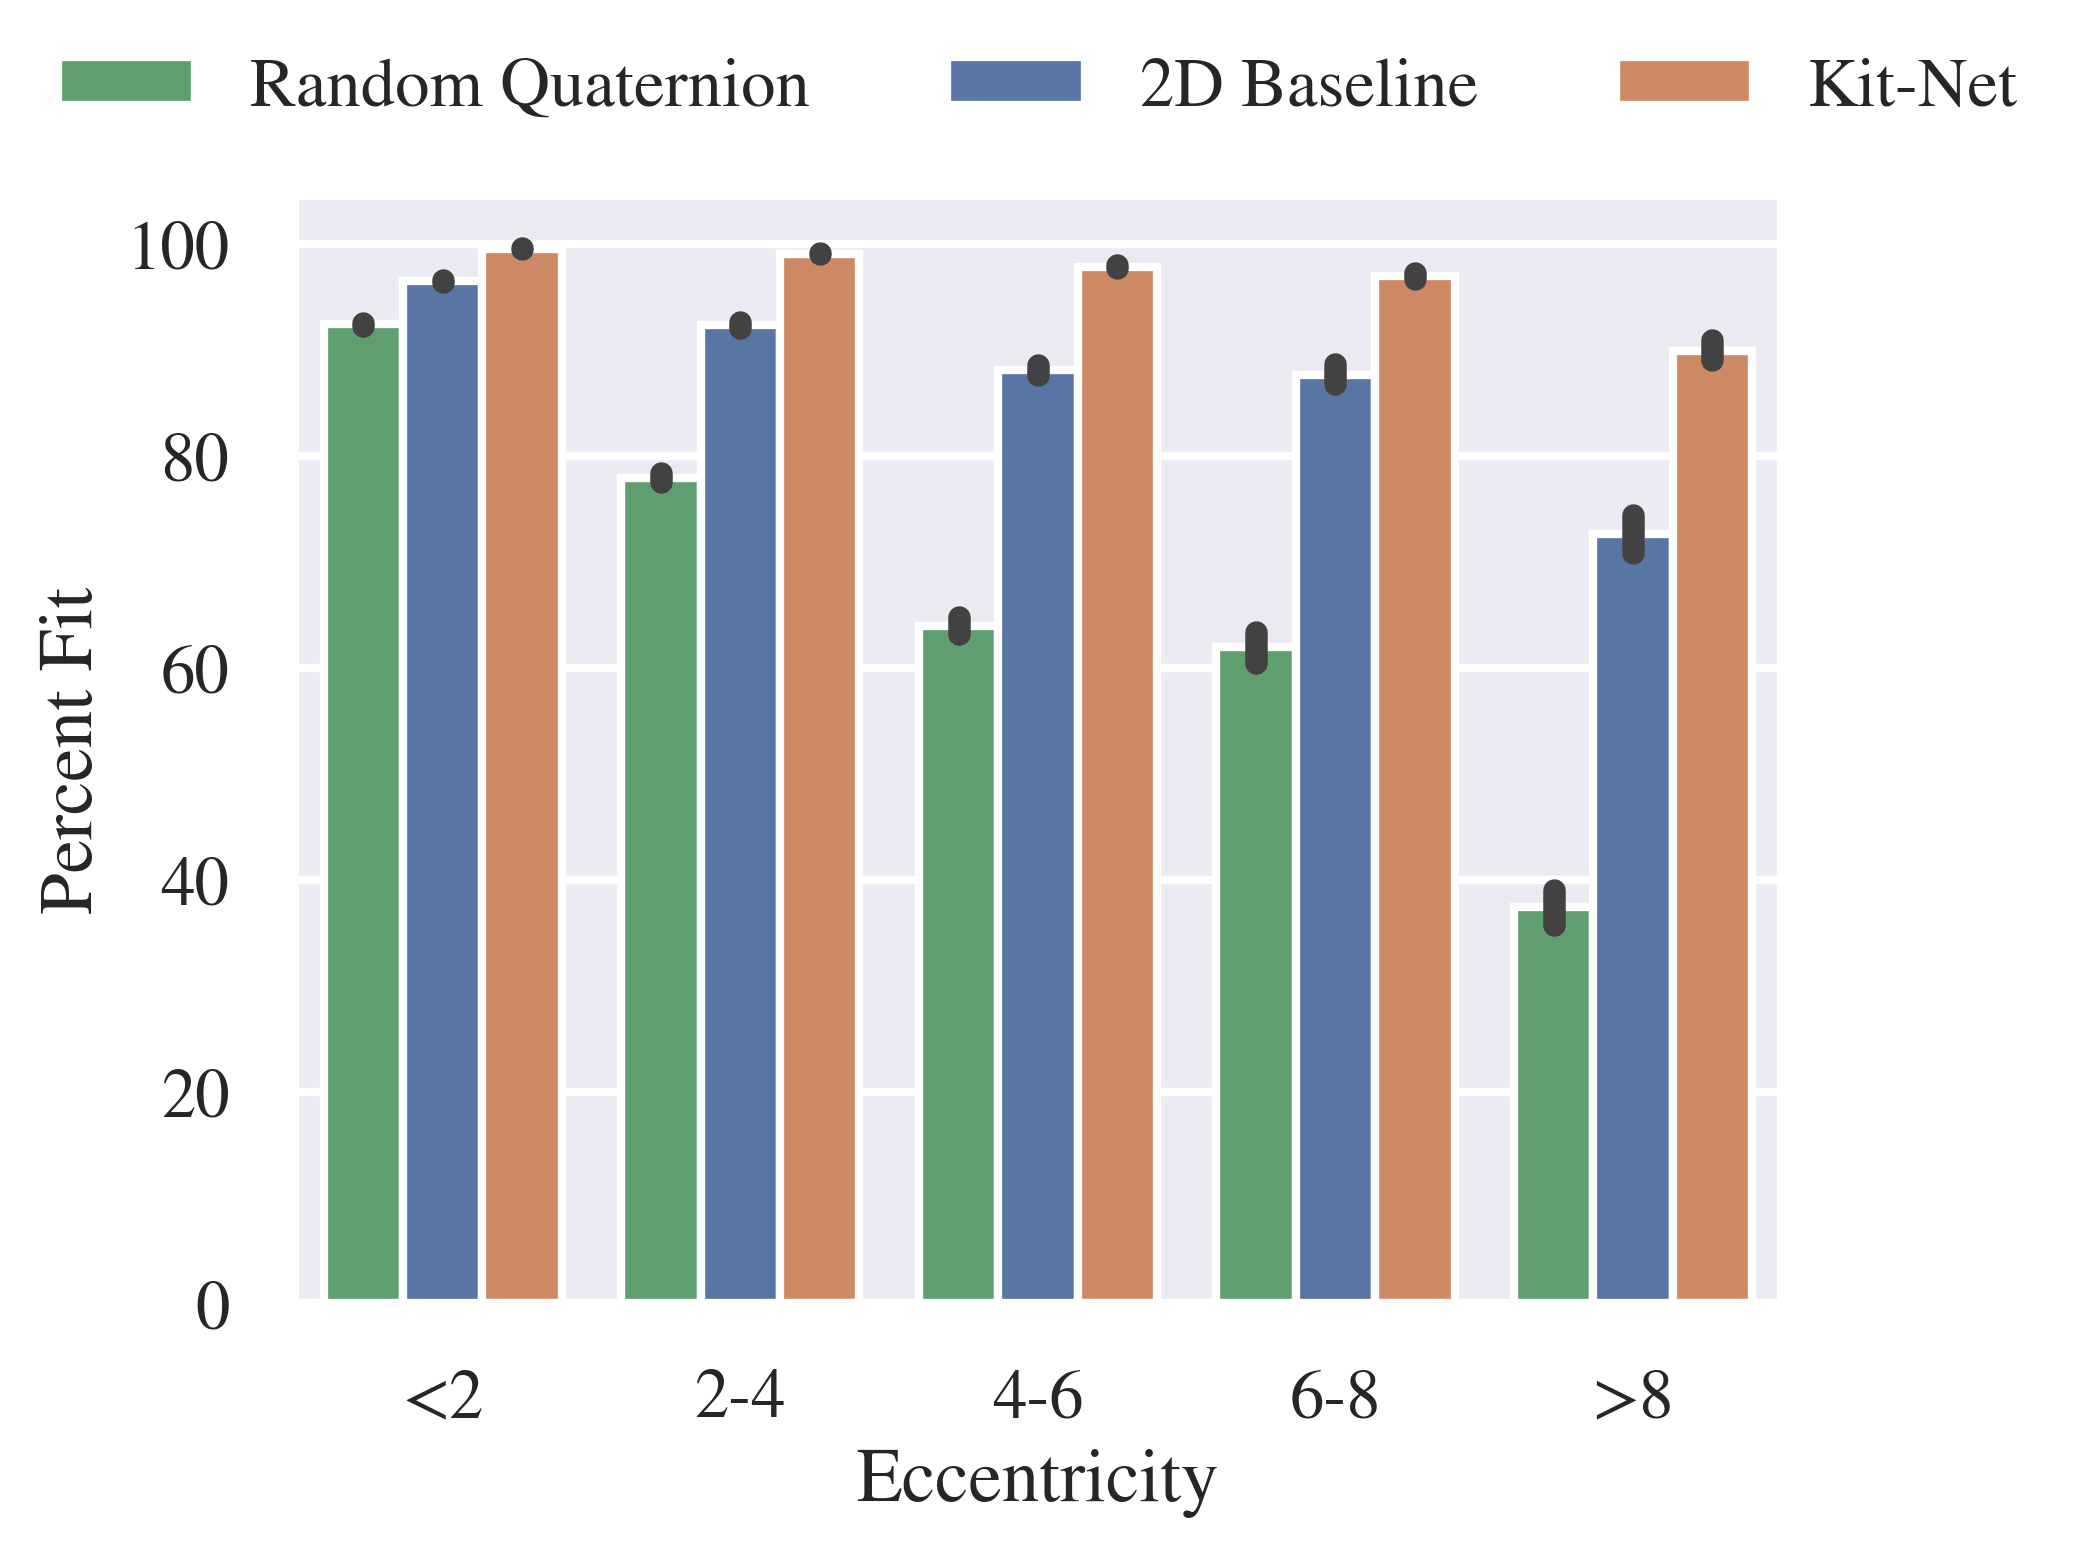
\includegraphics[width=\linewidth]{figures/percent_fit_ecc_v4.png}
  \caption{\textbf{Aligning Objects to Prismatic Cavities in Simulation: }We evaluate Kit-Nets ability to align objects with prismatic cavities under the percent fit metric introduced in Section~\ref{subsec:metrics} across 512 depth image pairs for each of 174 objects not seen during training. Given $(I^s,I^g)$, the network predicts $\hat{{_s}R^g}$ that will allow it to fit inside the cavity. We bin results by object eccentricity and observe that the mean percent fit decreases for objects of higher eccentricity. Kit-Net outperforms both the 2D and random baselines by a greater amount as object eccentricity increases.}
  \label{fig:mean-percent-fit-ecc}
\end{figure}

%  Figure~\ref{fig:percent-fit-runs} shows the progression of 16 runs of the controller on 4 randomly sampled  pairs for objects unseen in training and Figure~\ref{fig:percent-fit-hist} visualizes the distribution of fit percentages over 100 controller rollouts for each of the 4 eccentric objects visualized in Figure~\ref{fig:prism-task-eval-objects}. Results suggest that Kit-Net achieves a median final fit percentage of 99\%, suggesting that Kit-Net can effectively kit novel objects in novel prismatic cavities. \SD{Mike will add all the new Figures for eccentricity vs fit, controller rollout, controller histogram. Also baseline and then write about the figures here}

\begin{figure}[t]
  \centering % trim=left bottom right top, clip
%   \begin{tabular}{@{}c@{\enspace}c@{\enspace}c@{\enspace}c@{}}
%   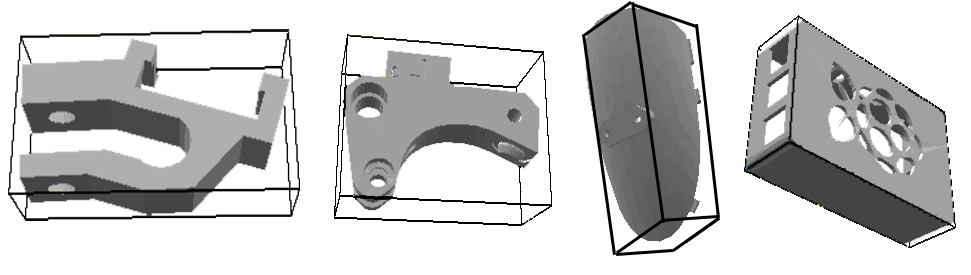
\includegraphics[height=54pt, trim=7 53 670 28, clip]{figures/Industrial Prismatic Cavity Task Objects.png} &
%   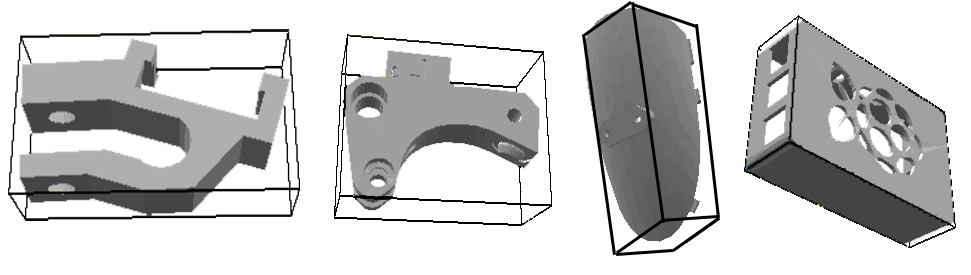
\includegraphics[height=54pt, trim=333 48 418 33, clip]{figures/Industrial Prismatic Cavity Task Objects.png} &
%   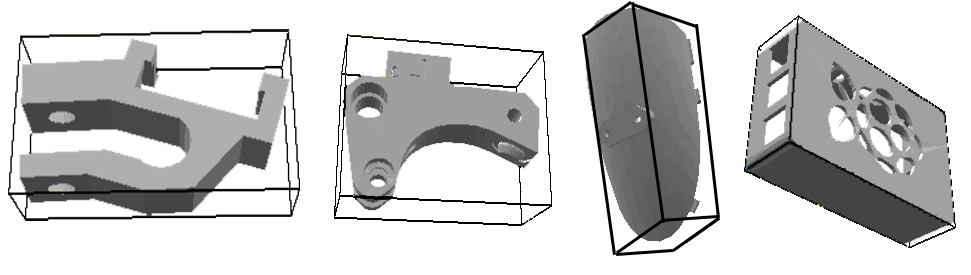
\includegraphics[height=54pt, trim=581 18 250 0, clip]{figures/Industrial Prismatic Cavity Task Objects.png} &
%   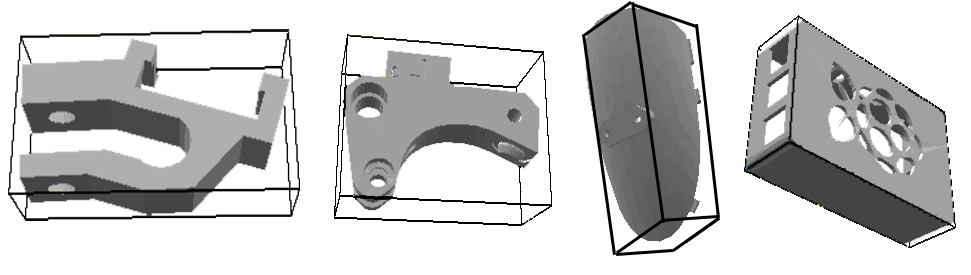
\includegraphics[height=54pt, trim=743 26 14 14, clip]{figures/Industrial Prismatic Cavity Task Objects.png} \\
%   \footnotesize Endstop holder &
%   \footnotesize Industrial part &
%   \footnotesize Shield part  &
%   \footnotesize Raspberry Pi case \\
%   \end{tabular}
  \subcaptionbox*{Industrial Part}{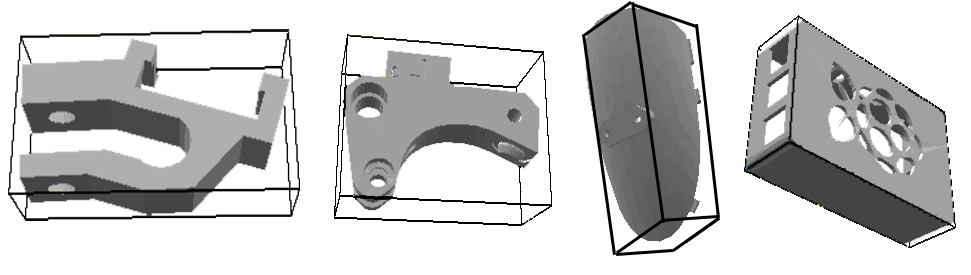
\includegraphics[height=50pt, trim=333 48 418 33, clip]{figures/Industrial Prismatic Cavity Task Objects.png}}%
  \hfill%
  \subcaptionbox*{Shield Part}[42pt]{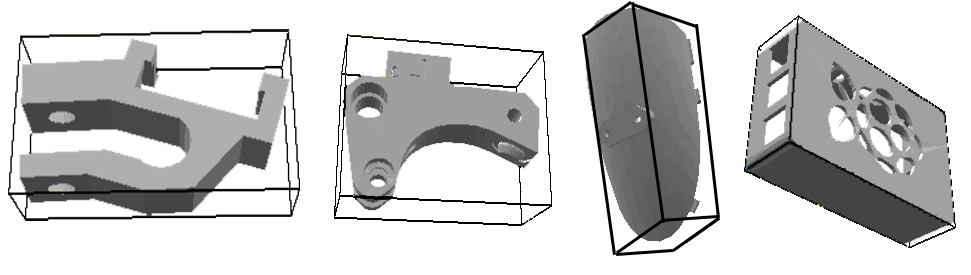
\includegraphics[height=50pt, trim=581 18 250 0, clip]{figures/Industrial Prismatic Cavity Task Objects.png}}%
  \hfill%
  \subcaptionbox*{Endstop Holder}{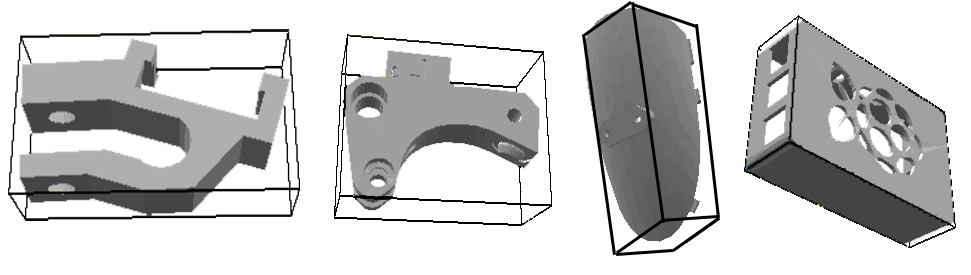
\includegraphics[height=50pt, trim=7 53 670 28, clip]{figures/Industrial Prismatic Cavity Task Objects.png}}%
  \hfill%
  \subcaptionbox*{Raspberry Pi Case}[62pt]{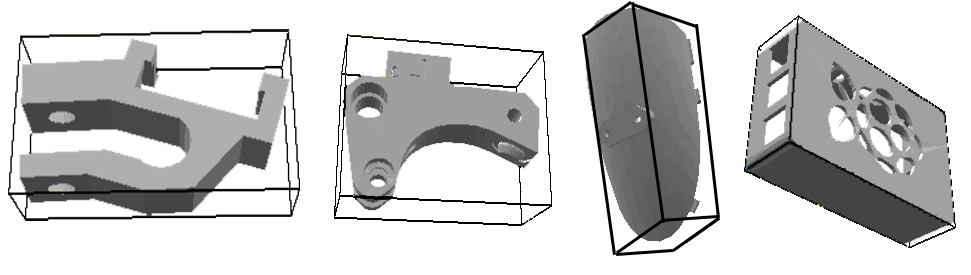
\includegraphics[height=50pt, trim=743 26 14 14, clip]{figures/Industrial Prismatic Cavity Task Objects.png}}
  \caption{\textbf{Examples of Novel Objects for Kit-Net Simulation Experiments: }
%   From left to right, these are the endstop holder, industrial part, shield part, and a raspberry pi case. 
  The four test objects are unseen during training and have eccentricity greater than 2, meaning their minimum volume bounding boxes are narrow and long. An outline of the corresponding minimum volume bounding box is shown around each part.}
  \label{fig:prism-task-eval-objects}
\end{figure}

\begin{figure}[t]
  \centering
  \vspace{8pt}
  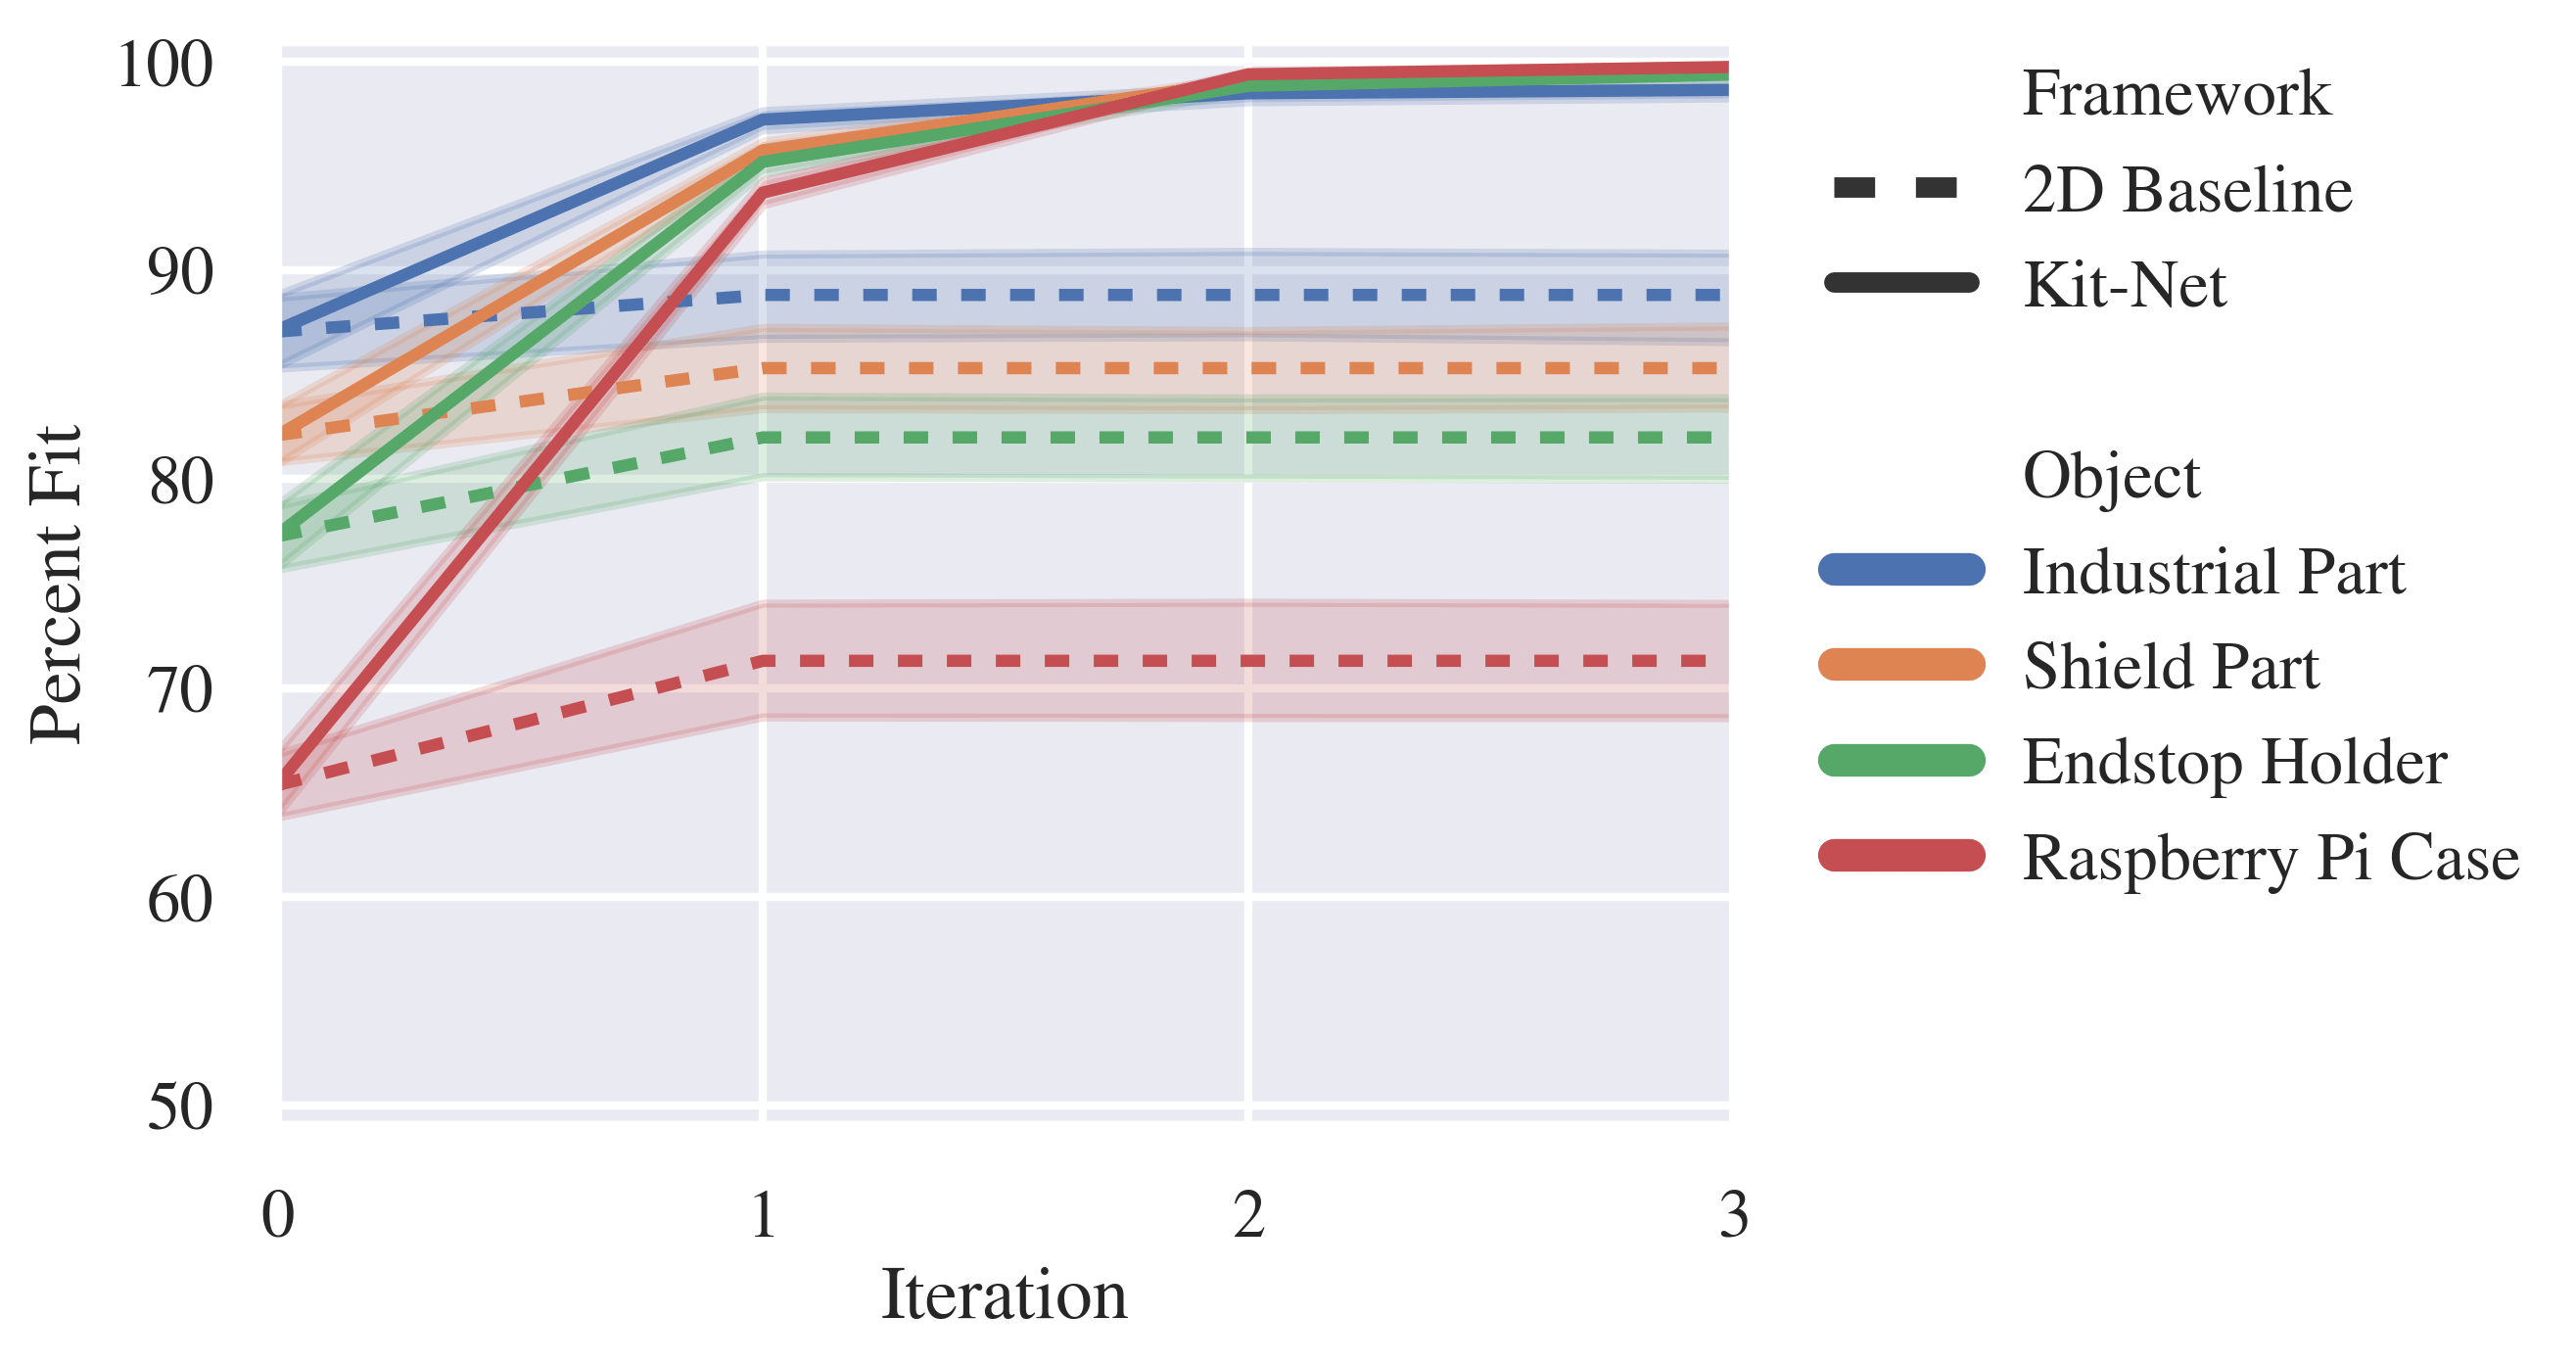
\includegraphics[width=0.48\textwidth]{figures/percent_fit_controller_runs_v6.png}
  \caption{\textbf{Kit-Net Simulation Results: } We visualize data from 100 runs on each of the 4 objects shown in Figure~\ref{fig:prism-task-eval-objects}. All objects require a 30\degree~rotation to be in alignment with the prismatic target at iteration 0, but their initial percent fits differ due to different eccentricities. Results suggest that Kit-Net is able to successfully align all 4 objects with their respective prismatic cavities while the baseline, which restricts itself to 2D rotations, performs significantly worse on all 4 objects.}
  \label{fig:percent-fit-runs}
\end{figure}



% \begin{figure}
%   \centering
%   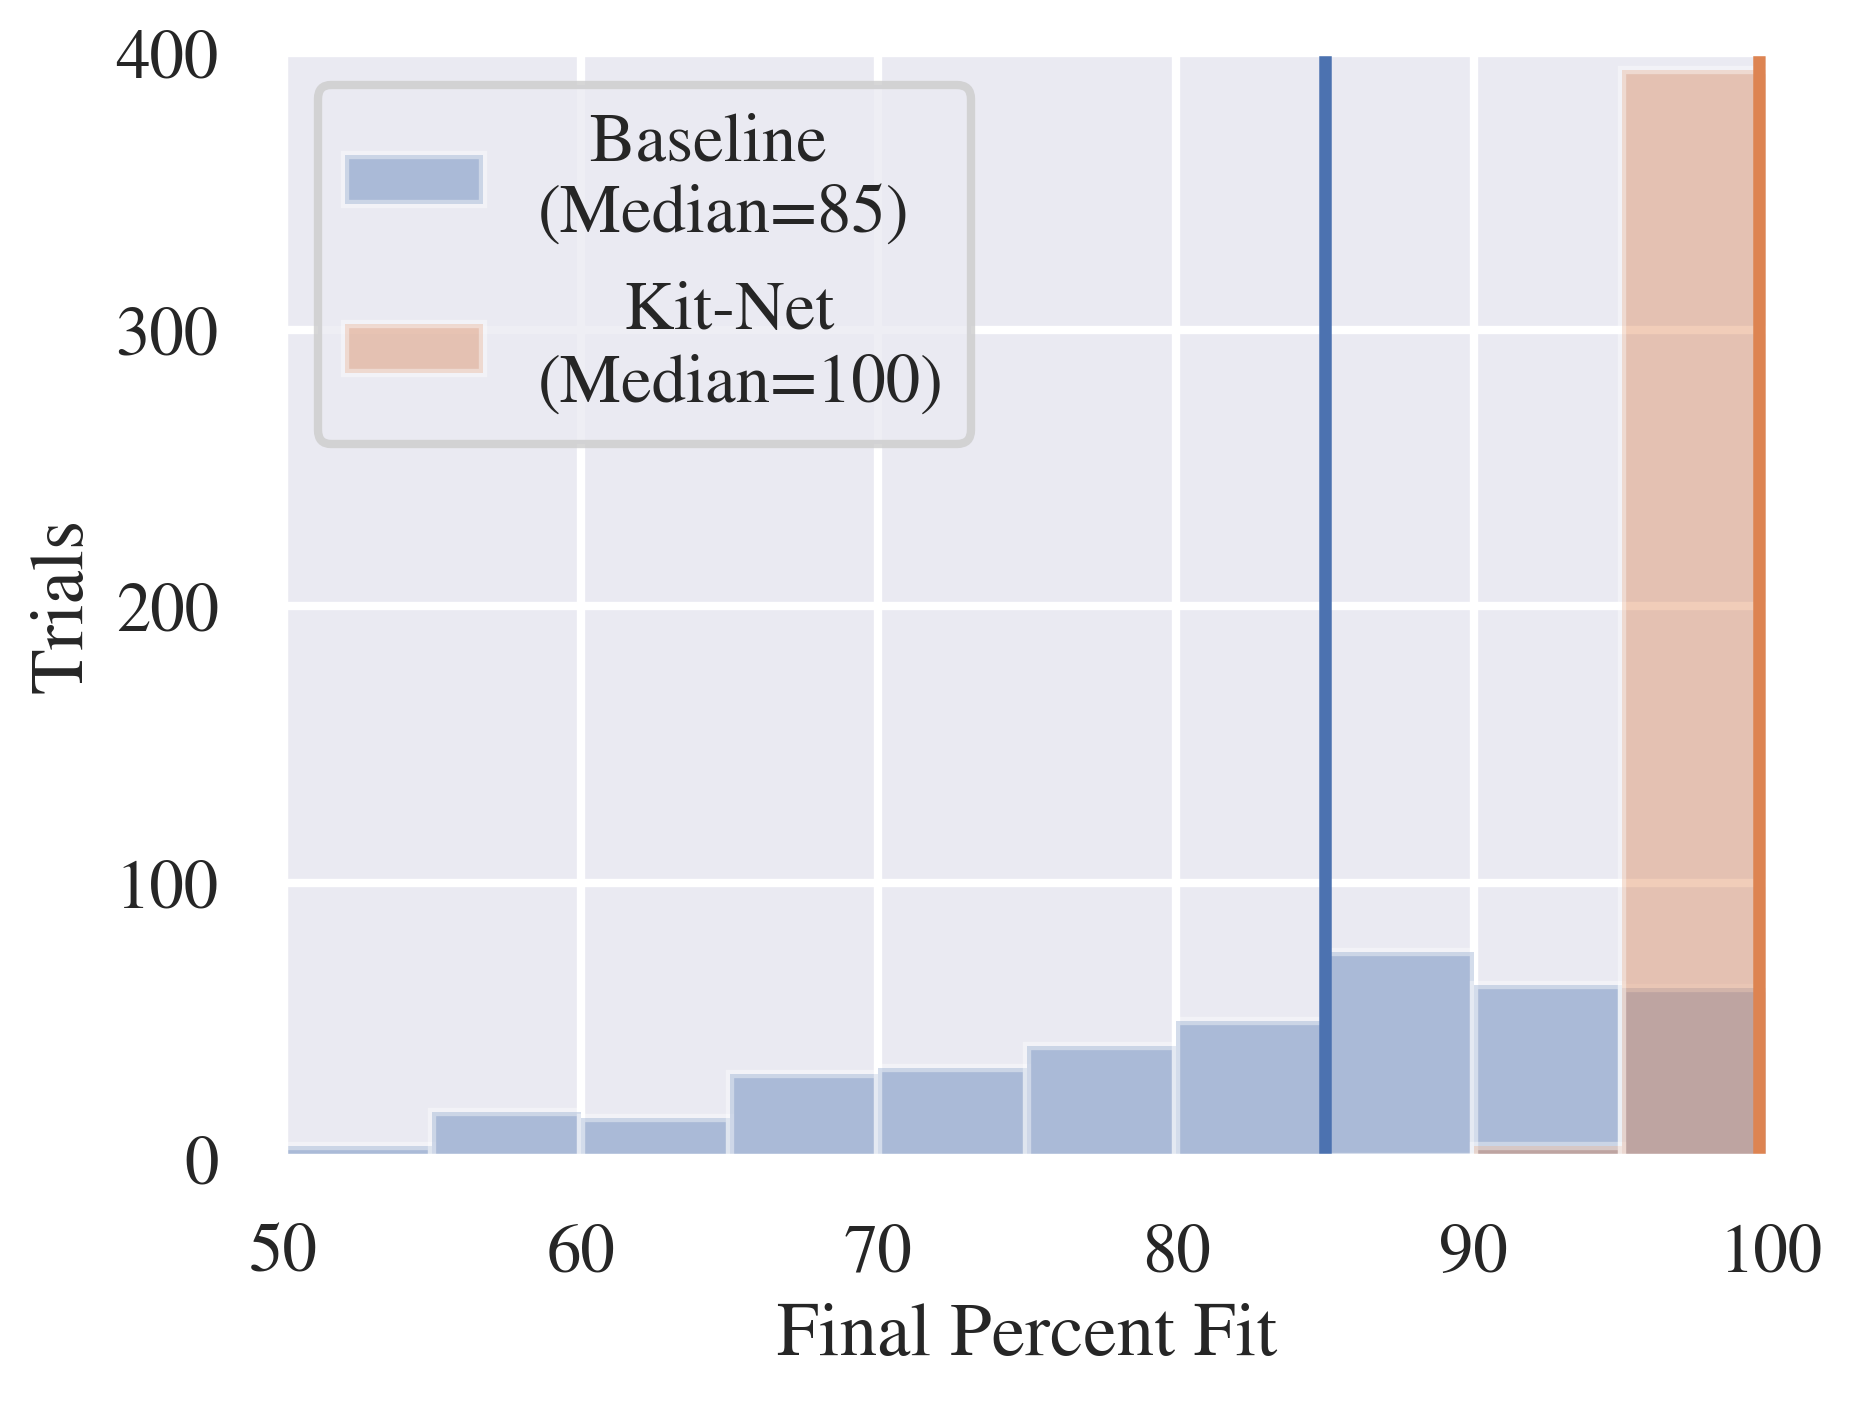
\includegraphics[width=0.9\linewidth]{figures/percent_fit_controller_hist_v3.png}
%   \caption{Kit-Net with the prismatic cavity targets. The controller takes incremental steps based on $\hat{{_s}R^g}$ and moves closer towards the target prism in up to 5 steps. We plot a histogram of the final percent fit and see that the median is 99.4\%, suggesting that Kit-Net can effectively orient novel objects towards a prismatic target for insertion. \AB{what information does this Figure provided that isn't already in Figure~\ref{fig:percent-fit-runs}?} \MD{agree, we can probably remove!}}
%   \label{fig:percent-fit-hist}
% \end{figure}
